% -*- root: 00-main.tex -*-
\section{Methods}
\label{sec:methods}
\subsection{Related work}\label{sec:related_work}
Previously, joint segmentation and registration have been applied successfully to other problems
such as longitudinal object tracking \citep{paragios_level_2003} and atlas-based
  segmentation \citep{gorthi_active_2011}.
The most common approach to solve the problem simultaneously is optimizing a deformation model
  (registration) that supports the evolution the active contours (segmentation), like
  \citep{paragios_level_2003,yezzi_variational_2003}.
\cite{unal_coupled_2005}, and later \cite{wang_joint_2006}, replaced the linear registration
  transform of \citep{yezzi_variational_2003} with a free-form deformation field.
\cite{droske_mumfordshah_2009} reviewed the existing techniques and proposed two different
  approaches for applying the Mumford-Shah functional \citep{mumford_optimal_1989} during simultaneous
  registration and segmentation by propagating the deformation field from
  the contours onto the whole image definition.
Recently, \cite{guyader_combined_2011} proposed a simultaneous segmentation and
  registration method in 2D using level sets and a nonlinear elasticity smoother on the
  displacement vector field, which preserves the topology even with very large deformations.
Finally, \cite{gorthi_active_2011} extended the existing methodologies using a multiphase
  level set function to register several active contours during the application
  of atlas-based segmentation.


\subsection{Registration framework and segmentation model derivation}\label{sec:methods_map}
Let $\gammaset_R = \{\Gamma_m: m \in \mathbb{N}, m \leq N_S\}$ be the set of $N_S$ surfaces
  extracted from the undistorted \gls*{t1} image (the reference space $R$).
We reformulate the segmentation of the distorted \gls*{dmri} images (the moving space $M$)
  as a registration problem where we search for an underlying deformation field $U$ such that
  the structures in $R$ defined by $\gammaset_R$ align optimally with their corresponding
  structures in $M$:

  \begin{align}
  U\colon R \subset \mathbb{R}^n &\to M \subset \mathbb{R}^n \notag\\
  \vec{r} &\mapsto \vec{r}' =\vec{r}+\vec{u}(\vec{r}),
  \label{eq:transform}
  \end{align}
  where $\vec{r}$ denotes a position in $R$, $\vec{r}'$ is
  its corresponding location in $M$, and $n$ denotes the dimensionality of images.
Finally, $\vec{u} = \vec{u}(\vec{r})$ is the displacement of every point with respect
  to the reference domain.
The general overview of how the surfaces interact with the registration framework
  is presented in \autoref{fig:method}.

\begin{figure}
  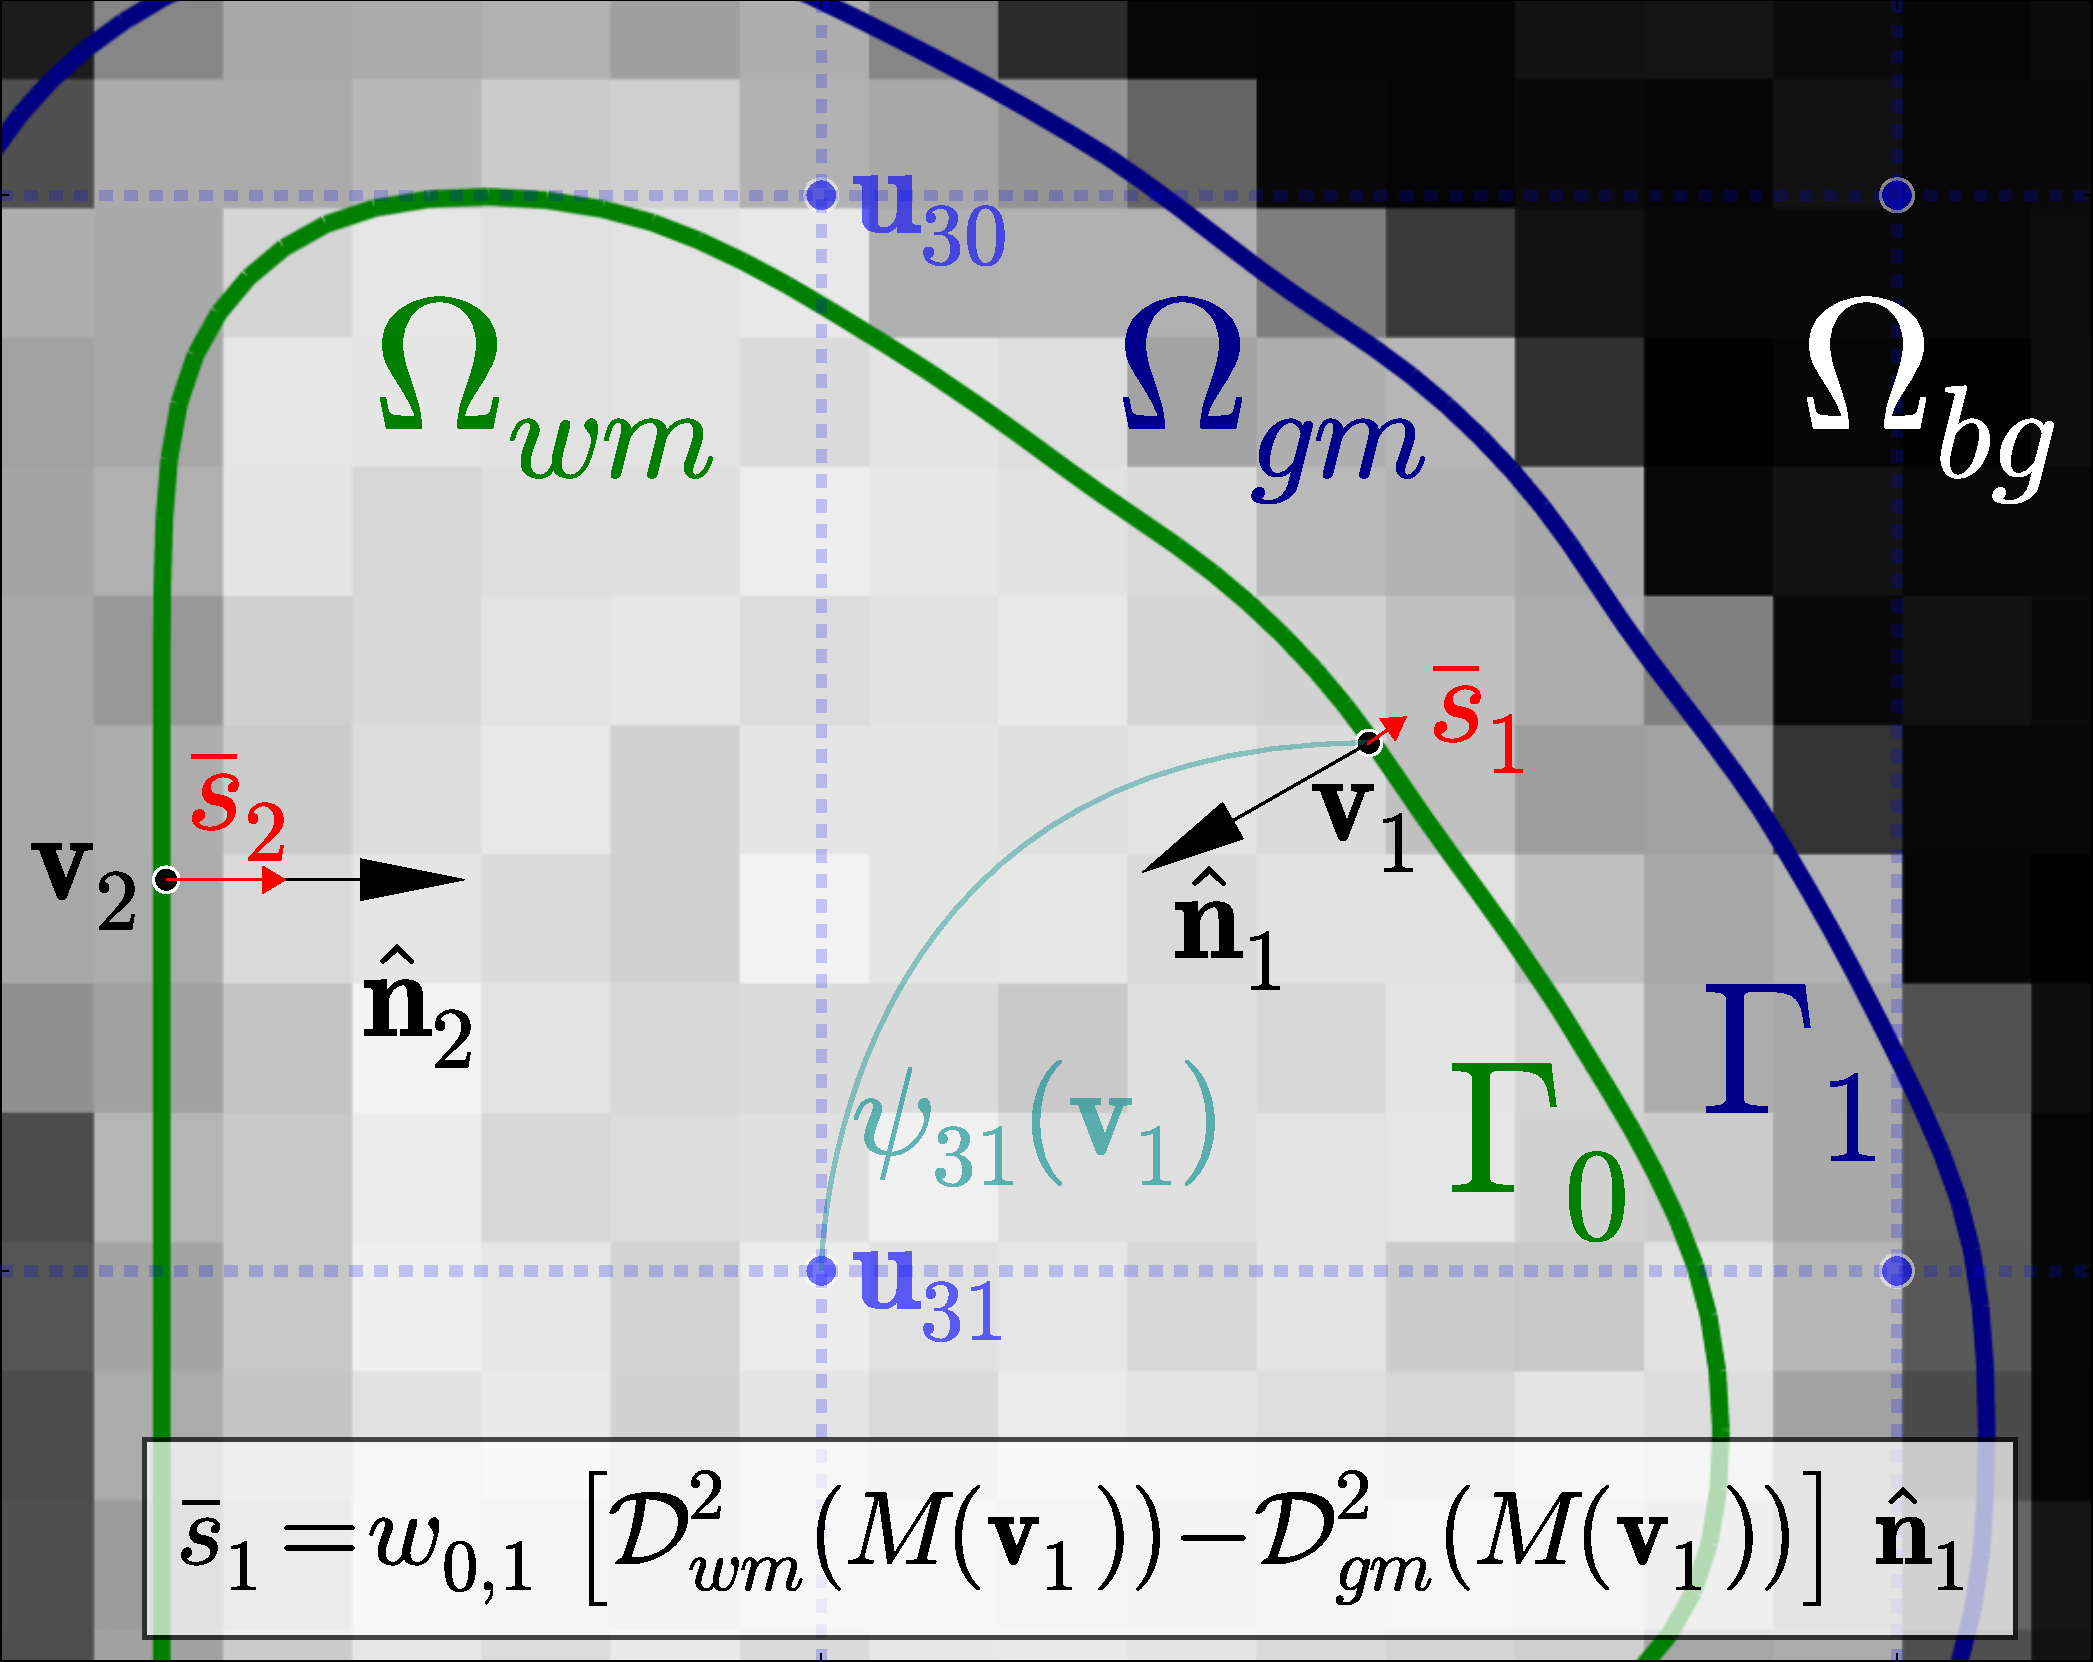
\includegraphics[width=\linewidth]{figure01}
  \caption{The active contours are defined as the interfacing surfaces of the competing
    \glspl{roi} $\Omega_i$, which
  are represented in green and dark blue in this close-up.
  They evolve iteratively following their inward normals $\hat{n}_i$ at each vertex
    $\vec{v}_i$ of the mesh.
  The gradient speeds $\bar{s}_i$ drive registration, which are computed as the disparity of the data
    energies with respect to the two limiting regions of $M(\vec{v}_i)$, the features of the image
    $M$ in the location of vertex $\vec{v}_i$ (see \suppl{equation SM5}).
  In this figure, $\bar{s}_1$ is written in the lower
    box, with $\Omega_{wm}$ in the inner limiting region, $\Omega_{gm}$ the outer region, and
    $w_{0,1}$ is the relative area associated with vertex $\vec{v}_1$ with respect to
    the total area of surface $\Gamma_0$.
      }\label{fig:method}
\end{figure}

\paragraph*{Cost-function derivation}
In a Bayesian framework for registration \citep{wyatt_map_2003,pohl_bayesian_2006,gass_simultaneous_2014},
  the mappings $U$ in \eqref{eq:transform} are
  evaluated based on their posterior probability given the observed data
  $M$.
Let $\omegaset = \{\Omega_l: l \in \mathbb{N}, l \leq N_L\}$ be the set of $N_L$ competing regions in
  which $M$ is partitioned by the projection of $\gammaset_R$.
Using Bayes' rule, the posterior likelihood is computed as:

  \begin{equation}
  P(U \mid M, \omegaset ) = \frac{P(M \mid U,\omegaset )\, P(U)}{P(M)},
  \label{eq:bayes_rule}
  \end{equation}
  where $P(M \mid U,\omegaset)$ is the data likelihood.
Because $\omegaset$ are mapped by $U$, then we simplify
  $P(U, \omegaset) = P(U) \implies P(M \mid U,\omegaset) = P(M \mid U)$.
The best estimate $\hat{U}$ then satisfies the maximum a posteriori criterion
  \citep{bishop_pattern_2006} and it aligns $\gammaset_R$ into $M$.
First, we assume independence between pixels, and thus we break down the
  global data likelihood into a product of pixel-wise conditional probabilities:

  \begin{equation}
  P(M \mid U) = \underset{l}{\prod} \underset{\vec{r}\in \Omega_l}{\prod}
    P\left( \vec{f}' \mid U \right),
  \label{eq:bayes_aposteriori}
  \end{equation}
  where $\vec{f}' = M(\vec{r}')$ is the feature vector at the displaced
  position $\vec{r}'$ \eqref{eq:transform} in the moving image.
For convenience and because it has been shown to be an appropriate approximation
  \citep{leemput_automated_1999,cuadra_comparison_2005}, we introduce two assumptions for each
  region $\Omega_l$:
  1) the features are i.i.d.; and 2) they can be modeled by multivariate normal
  distributions with the parameters $\lbrace \boldsymbol{\mu}_l, \boldsymbol{\Sigma}_{l} \rbrace$
  for each region $\Omega_l$.
Even though the features being segmented are not generally i.i.d., the spatial interdependency of
  voxels is implicitly supported by the piecewise smooth partition of the space \omegaset{}.
In \autoref{fig:model} it is shown that marginal distributions of data can be approximated by
  multivariate normal distributions. Therefore,

  \begin{align}
  P( M \mid U) &= \underset{l}{\prod} \underset{\vec{r} \in \Omega_l}{\prod}
  \mathcal{N} ( \vec{f} \mid \boldsymbol{\mu}_l, \boldsymbol{\Sigma}_{l} ) =   \underset{l}{\prod} \underset{\vec{r} \in \Omega_l}{\prod} \frac{1}{ \sqrt{(2\pi)^{C}\,\left|\boldsymbol{\Sigma}_{l}\right|}}\,{e^{\left(-\frac{1}{2}
  \mdist{f'}{l} \right)}},
  \label{eq:pdf}
  \end{align}
  using $\mdist{f}{l}$ to denote the squared \emph{Mahalanobis distance} of $\vec{f}$ with respect
  to the descriptors of region $l$ as
  $\mdist{f}{l} = (\vec{f} - \boldsymbol{\mu}_l)^T \, {\boldsymbol{\Sigma}_l}^{-1} \, (\vec{f} - \boldsymbol{\mu}_l)$.
$C$ is the number of channels comprised in the image $M$.
In fact, the projection of $\gammaset_R$ onto $M$ is an implicit segmentation model, for which
  the covariance matrix $\boldsymbol{\Sigma}_l$ of each region is minimized. In \autoref{fig:model},
  this minimization is illustrated for the segmentation of the \gls*{fa} and the \gls*{adc} maps
  of one subject.

\begin{figure}
\includegraphics[width=\linewidth]{figure04A}
\includegraphics[width=\linewidth]{figure04B}
\includegraphics[width=\linewidth]{figure04C}
\caption{%
Evolution of the segmentation model defined by the homogeneous regions $\Omega_i$
  for a real dataset.
Panel A shows how the \gls*{fa} and the \gls*{adc} are clustered by the surfaces mapped to
  $M$ through the ground-truth.
Panel B shows the same information at the initialization step of \regseg{}.
Since the surfaces are misaligned in $M$, the spreads of the sampled distribution for
  each region are large.
Panel C, after \regseg{} registration, shows how the covariance matrices $\boldsymbol{\Sigma}_l$
  are minimized with respect to panel B, and the resulting segmentation is close
  to the theoretical situation presented in panel A.
The left (large) plot in each panel represents a kernel density estimate of the location and spread of
  each region $\Omega_i$ in the bivariate feature space of $M$, which comprises
  the \gls*{fa} and \gls*{adc} maps.
At the top and the right margins, the marginal distributions of $\Omega_i$ are also plotted for
  the \gls*{fa} and \gls*{adc}, respectively.
On the right, the sampled distribution of each region is shown in small scatter plot, in contrast to
  the complete bivariate data.
}\label{fig:model}
\end{figure}

\paragraph*{Regularization}
The smoothness of the resulting displacements field is induced by a Thikonov regularization
  prior:

  \begin{align}
  P(U) = \underset{\vec{r}}{\prod}\, p(\vec{u}) &=
  \underset{\vec{r}}{\prod}\, p_0(\vec{u}) \, p_1(\vec{u}), \text{ with} \\
  p_0(\vec{u}) &= \mathcal{N}( \vec{u} \mid 0, \mathbf{A}^{-1}), \notag\\
  p_1(\vec{u}) &= \mathcal{N}(  \nabla \vec{u} \mid 0, \mathbf{B}^{-1}),
  \label{eq:thikonov}
  \end{align}
 which requires that the distortion and its gradient have zero
  mean and variance governed by the matrices $\mathbf{A}$ and $\mathbf{B}$.
Finally, the maximum a posteriori problem is adapted to a variational problem where we search for
  the minimum of an energy functional by applying $E(\vec{u}) = -\log \{P( M \mid U) \, P(U)\}$:

  \begin{align}
  E(\vec{u}) &= -\log \underset{l}{\prod}
  \underset{\vec{r} \in \Omega_l}{\prod}
  \mathcal{N} \left( \vec{f}' \mid \boldsymbol{\mu}_l, \boldsymbol{\Sigma}_l \right)\,p_0( \vec{u})\,p_1( \vec{u}) = \notag\\ &=
  \const + \underset{l}{\sum} \int_{\Omega_l} \mdist{f'}{l} \,d\vec{r} \, +   \int_{\Omega} \frac12 \left[ \vec{u}^T \mathbf{A} \vec{u} + (\nabla \vec{u})^T \mathbf{B} (\nabla \vec{u}) \right] \,d\vec{r}.
  \label{eq:energy}
  \end{align}
This expression is the dual of the Mumford-Shah functional that corresponds
  to the framework of \acrlong*{acwe} \citep{chan_active_2001}
  with the anisotropic regularization term of \cite{nagel_investigation_1986}.


\subsection{Numerical Implementation}
\label{sec:numerical_implementation}

\paragraph*{Deformation model}\label{sec:deformation_model}
Since the vertices of the surfaces $\{\vec{v}_i: \vec{v}_i \subset \gammaset \}_{i=1 \ldots N_V}$
  are probably located off-grid, it is necessary to derive $\vec{u}_i = \vec{u}(\vec{v}_i)$ from a discrete set of parameters
  $\{\vec{u}_k\}_{k=1 \ldots K}$.
Densification is achieved using a set of associated basis functions $\psi_k$ \eqref{eq:nodes_tfm}.
In our implementation, $\psi_k$ is selected as a tensor-product B-spline kernel
  of degree three.

  \begin{equation}
  \vec{v}_i' = \vec{v}_i + \vec{u}_i = \vec{v}_i + \sum_k \psi_k(\vec{r}) \: \vec{u}_k.
  \label{eq:nodes_tfm}
  \end{equation}


\paragraph*{Optimization}
\label{sec:gradient_descent}
To find the minimum of the energy functional \eqref{eq:energy},
  we propose a gradient-descent approach with respect to the underlying
  deformation field using the following \gls*{pde}:

  \begin{equation}
  \frac{\partial \vec{u}(\vec{r},t)}{\partial t} \propto - \frac{\partial E(\vec{u})}{\partial \vec{u}_k},
  \label{eq:general_gradient_descent}
  \end{equation}
  where $t$ is an artificial time parameter of the contour
  evolution and $\vec{u}_k$ are the parameters that support the estimate
  $\hat{U}$ of the transformation at the current time point.
Let us assume that the anisotropy is aligned with the imaging axes to simplify
  \eqref{eq:energy} as expression \eqref{eq:app_energy} in \ref{app:reg_term},
  and thus to compute its derivative \eqref{eq:general_gradient_descent}:

  \begin{align}
  \frac{\partial E(\vec{u})}{\partial \vec{u}_k} &=
  \frac{ \partial }{\partial \vec{u}_k} \Big\{
  \underset{l}{\sum} \int_{\Omega_l} \mdist{f'}{l} \,d\vec{r} \, +   \int_{\Omega} \frac12 [ \boldsymbol{\alpha} \cdot \vec{u}^{\circ2}
  + \boldsymbol{\beta} \cdot (\nabla \vec{u})^{\circ2} ] \,d\vec{r}
  \Big\},
  \label{eq:gradient_descent}
  \end{align}
  where $\vec{u}^{\circ2} = \vec{u}^T \cdot \vec{u}$.
Then, the data and regularization terms are split and discretized to compute their
  derivatives.
The computation of the explicit shape gradients at each $\vec{v}_i'$ is illustrated in \autoref{fig:method}.
Then, \eqref{eq:gradient_descent} can be reformulated as (see \suppl{equations SM6-SM12}):

  \begin{align}
  \frac{\partial E(\vec{u})}{\partial \vec{u}_k} &=
  \vec{g}_k  + \boldsymbol{\alpha} \cdot \vec{u}_k - \boldsymbol{\beta} \cdot (\Delta \vec{u}_k).
  \label{eq:final_gradient}
  \end{align}

Finally, to descend this gradient, we establish a semi-implicit Euler scheme (see \suppl{section S1.3}),
  with a step size parameter $\delta$, which we solve in the spectral domain as follows:

  \begin{align}
  \vec{u}_k^{t+1} = \mathcal{F}^{-1}\left\{ \frac{\mathcal{F}\{\delta^{-1} \, \vec{u}_k^t - \vec{g}_k\} }                  {\mathcal{F}\{(\delta^{-1} + \boldsymbol{\alpha})\, I - \boldsymbol{\beta}\Delta\}} \right\},
  \label{eq:update_equation}
  \end{align}
  where $I$ denotes the identity operator.


\paragraph*{Implementation details, settings, and convergence}
\label{sec:conv_report}
The \regseg{} tool includes a multiresolution strategy on the free-form deformation field.
Registration pyramids are created by setting the spacing between the control points of the B-spline basis
  functions for each level of the multiresolution strategy.
The implementation details as well as other features (such as the sparse matrix approach
  to fast interpolation) and the main parameters
  (such as $\delta$, $\boldsymbol{\alpha}$, $\boldsymbol{\beta}$, the B-spline grid resolutions,
 and target image smoothing) are discussed in \suppl{section S1}.
The actual choices of the parameter settings are publicly distributed with the source code for the experiments.
The final settings were obtained manually based on feedback from the post-registration convergence
  reports (such as that found in \suppl{section S1.3}).
We released \regseg{} along with the tool to generate the convergence report.

\subsection{Evaluation protocol}\label{sec:evaluation_protocol}
In order to assess the performance of \regseg{}, we defined the following general
  evaluation protocol:
1) Extract the set of undistorted surfaces $\gammaset_R$;
2) Compute a ground-truth field of displacements $U_\text{true}$, which is applied to
  generate warped images ($M$) for segmentation;
3) Execute \regseg{} with $\gammaset_R$ and use the warped data as inputs; and
4) Perform a visual assessment and compute the error metrics.

The adaptation of this protocol to the simulated phantoms and real data is explained in the
  following sections.
A first proof of concept to demonstrate \regseg{} in phantoms with simple
  geometries is introduced, using $U_\text{true}$ without directional restrictions.
Then, a more realistic environment with $U_\text{true}$ restricted to the
  \gls*{pe} axis of real \gls*{dmri} datasets is presented.

\subsection{Simulated phantoms}\label{sec:digital_phantoms}
The workflow required to simulate the digital phantoms and to assess the performance of
  \regseg{} with them is presented in \autoref{fig:evphantoms}.
A set of four binary objects (i.e., ``box'', ``ball'', ``L'',
  and ``gyrus'') was generated by combining the binarization of
  analytical shapes and mathematical morphology.
The reference surfaces $\gammaset_R$ were extracted from the binary shapes
  using \emph{FreeSurfer} tools \citep{fischl_freesurfer_2012}.
The ground-truth distortion was generated using a chain of two displacement
  fields supported by grids of B-spline basis functions.
The coefficients of the basis functions were generated randomly for
  both levels in their three dimensions.
The three components of the displacements $\vec{u} = (u_d)$
  were bounded above by 40\% of the separation between the control points
  at each level to obtain diffeomorphic transforms
  after concatenation \citep{rueckert_diffeomorphic_2006}.
The first deformation field was applied to generate large warpings
  with control points separated by 50.50 mm in the three dimensions
  ($u_d\leq$ 20.20 mm).
With the second warping, we aimed to obtain a field with smoothness
  close to that found in a typical distortion field of \gls*{dmri} data
  \citep{irfanoglu_susceptibility_2011}.
Therefore, the control points were separated by 25.25 mm ($u_d\leq$ 10.10 mm).
After generating the ground-truth deformation, the original surfaces
  were warped by interpolating the displacements field at each vertex.
The warped surfaces $\gammaset_\text{true}$ were binarized to generate tissue fractions
  at low (\isores[mm]{2.0}) and high (\isores[mm]{1.0}) resolutions.
Using a \gls*{mr} simulator \citep{caruyer_phantomas_2014}, we synthesized
  \gls*{t1} (TE/TR= 10/1500 ms) and \gls*{t2} images (TE/TR= 90/5000 ms), which
  corresponded to each phantom type, with each at two resolutions
  (1.0 mm and 2.0 mm isotropic).
The field of view at both resolutions was \isores[mm]{100}.
Next, \regseg{} was applied to map $\gammaset_R$ onto the warped phantoms to
  obtain the registered surfaces ($\hat{\gammaset}_\text{test}$).
To quantify the misregistration error, we computed the Hausdorff distance between
 $\hat{\gammaset}_\text{test}$ and $\gammaset_\text{true}$ using \citep{commandeur_vtk_2011}.

\begin{figure*}
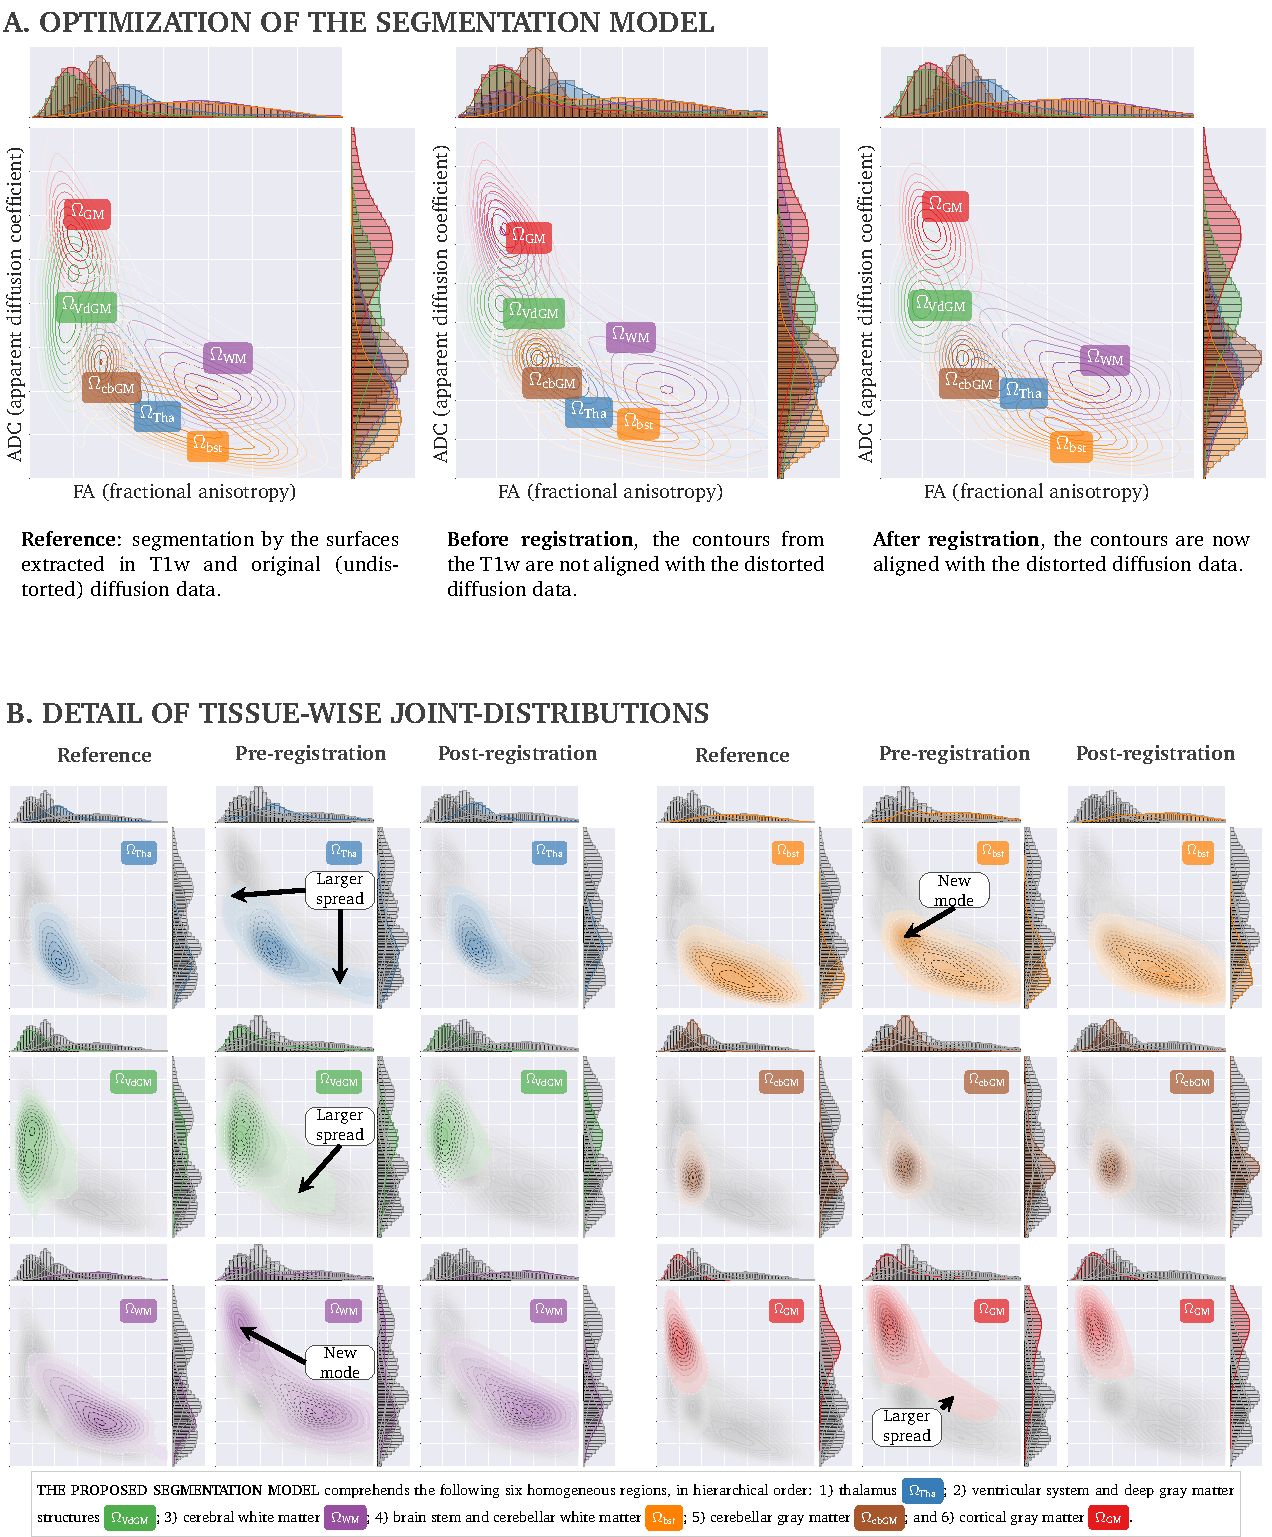
\includegraphics[width=\linewidth]{figure02}
\caption{Evaluation of \regseg{} using phantom data according to the following instrumental workflow.
  1) The reference surfaces $\gammaset_R$ are triangularized meshes extracted from the four binary shapes (i.e., ``box'', ``ball'', ``L'', ``gyrus'').
  2) A ground-truth displacement field was generated as described in \autoref{sec:digital_phantoms}, and applied to warp
      $\gammaset_R$, thereby obtaining $\gammaset_\text{true}$.
  3) After being warped, $\gammaset_\text{true}$ were projected onto the corresponding discrete 3D volume and downsampled to create partial volume effects at two resolutions,
     i.e., \isores[mm]{2.0} and \isores[mm]{1.0}, thereby producing sets of tissue fractions maps.
  4) The tissue fractions were fed into a \acrfull*{mr} simulator, which generated \acrfull*{t1} and \acrfull*{t2} -like images at the
     two possible resolutions.
  5) The \regseg{} tool was applied using the warped test images as multispectral moving images and $\gammaset_R$ as shape priors.
  6) The agreement between the surfaces fitted by \regseg{} ($\hat{\gammaset}_\text{test}$) and $\gammaset_\text{true}$ were assessed
     visually using automatically generated visual reports and quantitativelly with the Hausdorff distance between the
     corresponding surfaces.}\label{fig:evphantoms}
\end{figure*}


\subsection{Real datasets} \label{sec:human_connectome}
The general experimental framework for the real datasets is presented in \autoref{fig:evworkflows},
which extends our previous evaluation \citep{esteban_simulationbased_2014} of distortions
  using \gls*{dmri} phantoms.

\begin{figure*}
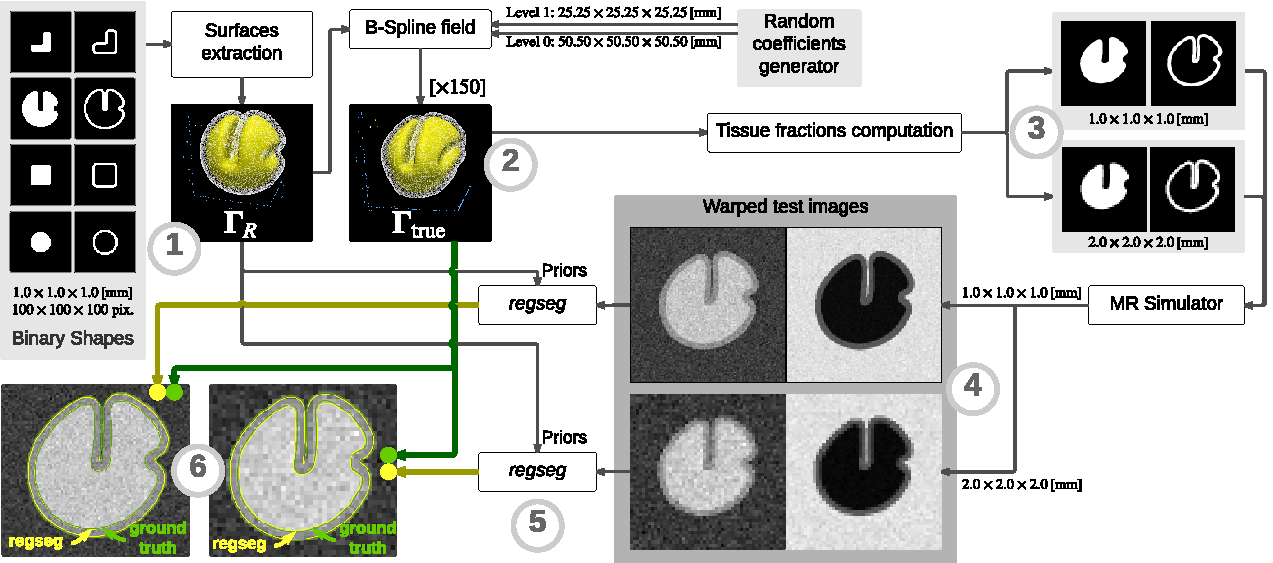
\includegraphics[width=\linewidth]{figure03}
\caption{Experimental workflow employed to process real data from the \acrfull*{hcp}.
  1) $\gammaset_R$ were extracted from the anatomical reference (\gls*{t1} image).
  2) For use as the ground truth, we generated a plausible synthetic distortion $U_\text{true}$
    from the field map with \eqref{eq:fieldmap}.
  3) The \gls*{dmri} data were warped using $U_\text{true}$ to reproduce the effects of real
    susceptibility-derived distortions.
  Target diffusion scalars (\gls*{fa} and \gls*{adc}) were computed with the distorted data and
    stacked to feed the multivariate input required by \regseg{}.
  4) The method was run to obtain $U_{test} = \hat{U}_{true}$, i.e., the estimate of
    the ground-truth deformation.
  5) The results were evaluated visually and quantitatively.}\label{fig:evworkflows}
\end{figure*}


\paragraph*{Data}
To evaluate \regseg{} using real \gls*{dmri} data obtained from human brains,
  we collected 16 subjects from the \gls*{hcp} database.
The original acquisitions are released within ``unprocessed'' packages, whereas
  the ``minimally preprocessed'' packages contain the corresponding images after
  some processing (correction for several artifacts, brain-extraction, spatial
  normalization, etc.).
We refer the reader to \citep{essen_human_2012} for exact details of the acquisition
  parameters and \citep{glasser_minimal_2013} for the preprocessing issues.
These datasets comprise a large set of images, including \gls*{t1}, \gls*{t2}, and
  multi-shell \gls*{dmri} images.

\paragraph*{Segmentation model}
Based on our experience % \citep{esteban_brain_2012}
  and previous studies \citep{ennis_orthogonal_2006},
  we defined the moving image as a stack of the \gls*{fa} and \gls*{adc} maps derived
  from \gls*{dmri} data.
After evaluating several alternative models, we empirically defined a partition \omegaset{}
  according to the following six regions:
  1) thalamus ($\Omega_{Tha}$);
  2) ventricular system and deep \gls*{gm} structures ($\Omega_{VdGM}$);
  3) cerebral \gls*{wm} ($\Omega_{WM}$);
  4) brain stem and cerebellar \gls*{wm} ($\Omega_{bst}$);
  5) cerebellar \gls*{gm} ($\Omega_{cbGM}$); and
  6) cortical \gls*{gm} ($\Omega_{GM}$).
Using tools in \emph{FreeSurfer} and appropriate selections of labels in the
  \emph{aparc} segmentation released with the \gls*{hcp} data, we extracted the $\gammaset_R$ set for the
  reference surfaces.
The segmentation model corresponding to this partition is shown in \autoref{fig:model}
  and discussed in greater detail in \suppl{section S4}.

\paragraph*{Ground-truth generation}
Realistic deformation is achieved by generating displacements fields that satisfy the theoretical
  properties of distortion \citep{jezzard_correction_1995}.
The displacements along the \gls*{pe} axis of the \gls*{dmri} image are related to the local
  deviation of the field $\Delta B_0(\vec{r})$ from its nominal value $B_0$, as follows:

  \begin{equation}
  u_\text{PE} = \frac{\gamma \, T_{acq}\, s_\text{PE}}{2\pi}\Delta B_0(\vec{r})\text{ [mm]},
  \label{eq:fieldmap}
  \end{equation}
where $\gamma$ is the gyromagnetic ratio, $T_{acq}$ is the readout time, and
  $s_\text{PE}$ is the pixel size along \gls*{pe}.
Certain \gls*{mr} sequences are designed to estimate $\Delta B_0$, thereby obtaining
  the so-called field map.
We derived the deformation $U_\text{true}$ from the field map image released with
  the corresponding packages of each dataset in the \gls*{hcp}.
The field map was unwrapped\footnote{fieldmaps are phase maps, which are intrinsically clipped in the interval
  of $[-\pi, \pi)$ [rads] or [rads/s].} and smoothed before applying \eqref{eq:fieldmap}.
Next, the original \gls*{dmri} was warped using the resulting displacement field and fed into
  a pipeline to process the corresponding \gls*{dti}, thereby computing the derived scalars of
  interest (\gls*{fa} and \gls*{adc}) using \emph{MRtrix} \citep{tournier_mrtrix_2012}.

\paragraph*{Metric assessment}
Initially, we investigated the appropriateness of the segmentation model.
For five test datasets, we uniformly sampled the space of distortions
  $\hat{U} = \epsilon \cdot U_\text{true} = \vec{r} + \epsilon \, u_\text{PE}$
  (with $\epsilon \in [-1.1, 1.1]$ and $u_\text{PE}$ from \eqref{eq:fieldmap}),
  and we evaluated the data term of the cost function \eqref{eq:energy}.
The minimum of the cost function (\autoref{sec:methods_map}) was consistently located at
  $\epsilon=0.0$ (the ground-truth) for all of the cases (\suppl{Figure S2}).

\paragraph*{Cross-comparison}
A similar workflow to the general evaluation framework used for \autoref{fig:evworkflows}
  was employed to integrate the alternate \gls*{t2b} registration scheme.
We reproduced the solution and settings provided with \emph{ExploreDTI}
  \citep{leemans_exploredti_2009}, which is a widely used toolkit for tractography analysis of
  \gls*{dti}.
\emph{ExploreDTI} internally employs \emph{elastix} \citep{klein_elastix_2010} to
  perform registration.

\paragraph*{Error measurement}\label{sec:experiments_evaluation}
Distortion only occurs along the \gls*{pe} axis of the image, so we computed the
  \gls*{swindex} as the area-weighted distance between the corresponding vertices of
  $\gammaset_{true}$ and their estimate obtained by the method under the test $\hat{\gammaset}_\text{test}$:

  \begin{equation}
  sWI = \frac{1}{\sum_i a_i} \sum\limits_i^{N_V} a_i\,\|
  \vec{v}_i - \hat{\vec{v}}_i \|,
  \label{eq:swindex}
  \end{equation}
  where $\vec{v}_i \subset \gammaset_\text{true}$ are the locations of the total $N_V$ vertices
  and $\hat{\vec{v}}_i \subset \hat{\gammaset}_\text{test}$ are the recovered locations
  that correspond to $\vec{v}_i$.
In practice, we only report the \gls*{swindex} for three surfaces of crucial interest in whole-brain
  tractography.
These three surfaces delineated the following regions in the model: $\Omega_{VdGM}$, $\Omega_{WM}$, and $\Omega_{GM}$.